


\frame{
\begin{block}{}
\begin{itemize}
\item The computational procedures used in computer software for the evaluation of a library function, such as $\sin(x)$, $\cos(x)$, or $e^x$, involve polynomial appproximation. 
\item The state-of-the-art methods use rational functions ( which are the quotients of polynomials ). 
\end{itemize}
\end{block}
\begin{center}
$\Downarrow$
\end{center}
\begin{block}{}
However, the theory of polynomial approximation is suitable for a first course in numerical analysis. 
In this chapter we develop the basic theory needed to investigate these matters. 
\end{block}
}

\frame{
\begin{block}{}
Suppose that the function $f (x) = e^x$ is to be approximated by a polynomial of degree $n = 2$ over the interval $[-1,1]$. 
\end{block}
\begin{figure}
\begin{center}
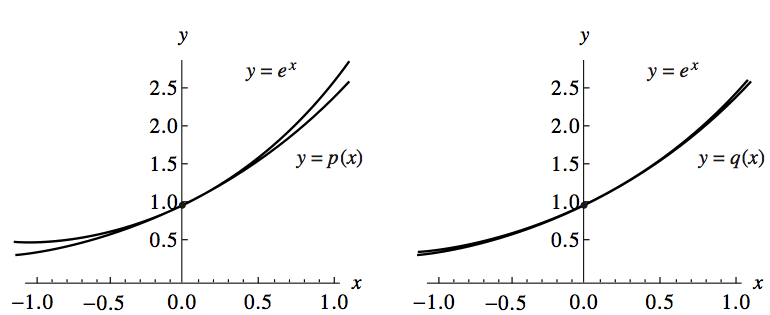
\includegraphics[width=90mm]{chap-3/fig_4-1.png}
\end{center}
\end{figure}
\begin{itemize}
\item The Taylor polynomial is shown in left figure  and can be contrasted with the Chebyshev approximation in right figure. 
\item The maximum error for the Taylor approximation is $0.218282$, whereas the maximum error for the Chebyshev polynomial is $0.056468$. 
\end{itemize}
}

\frame{
\frametitle{An associated problem}
\framesubtitle{ involves construction of the collocation polynomial.}
\begin{block}{}
Given $n + 1$ points in the plane (no two of which are aligned vertically),
\end{block}
\begin{center}
$\Downarrow$
\end{center}
\begin{block}{}
The collocation polynomial is the unique polynomial of degree $\le n$ that passes through the points. 
\end{block}
}

\frame{
%\item In cases where data are known to a high degree of precision, the collocation polynomial is sometimes used to find a polynomial that passes through the given data points. 
\begin{block}{A variety of methods can be used to construct the collocation polynomial : }
\begin{itemize}
\item solving a linear system for its coefficients, 
\item the use of Lagrange coefficient polynomials, 
\item the construction of a divided differences table and the coefficients of the Newton polynomial. 
\end{itemize}
\end{block}
}

\frame{
\frametitle{For example}
\framesubtitle{例子}
 the collocation polynomial of degree $n = 4$ that passes through the five points $(1,2)$, $(2,1)$, $(3,5)$, $(4,6)$, and $(5,1)$ is 
\begin{equation*}
P(x) = \frac{5x^4 - 82x^3 + 427x^2 - 806x + 504}{24}
\end{equation*}
and a graph showing both the points and the polynomial is given in the following figure.
\begin{figure}
\begin{center}
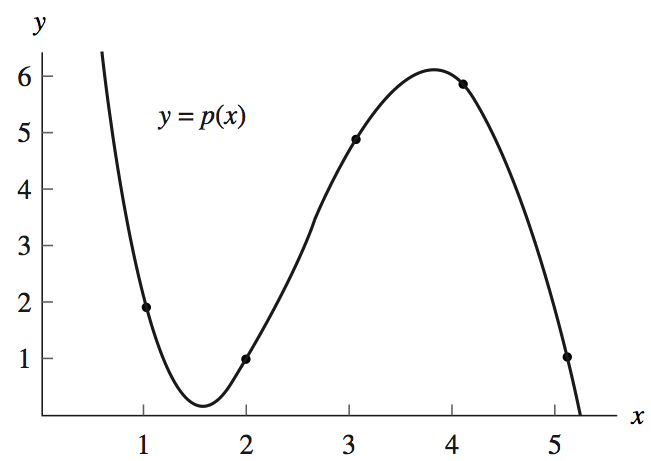
\includegraphics[width=50mm]{chap-3/fig_4-2.png}
\end{center}
\end{figure}
}


